\documentclass[a4paper,11pt]{article}

%%%%%%%%%%%%%%%%%%%%%%%%%%%%%%%%%%%%%%%%%%%%%%%%%%%%%%%%%%%%%%%%%%%%%%%%
% Paquetes utilizados
%%%%%%%%%%%%%%%%%%%%%%%%%%%%%%%%%%%%%%%%%%%%%%%%%%%%%%%%%%%%%%%%%%%%%%%%

% Gráficos complejos
\usepackage{graphicx}
\usepackage{subfig}
\usepackage{placeins}

% Soporte para el lenguaje español
\usepackage{textcomp}
\usepackage[utf8]{inputenc}
\usepackage[T1]{fontenc}
\DeclareUnicodeCharacter{B0}{\textdegree}
\usepackage[spanish]{babel}

% Código fuente embebido
\usepackage{listings}

% PDFs embebidos para el apéndice
\usepackage{pdfpages}

% Matemáticos
\usepackage{amssymb,amsmath}

% Formato de párrafo
\setlength{\parskip}{1ex plus 0.5ex minus 0.2ex}

%%%%%%%%%%%%%%%%%%%%%%%%%%%%%%%%%%%%%%%%%%%%%%%%%%%%%%%%%%%%%%%%%%%%%%%%
% Título
%%%%%%%%%%%%%%%%%%%%%%%%%%%%%%%%%%%%%%%%%%%%%%%%%%%%%%%%%%%%%%%%%%%%%%%%

% Título principal del documento.
\title{\textbf{Trabajo Práctico 0: Infraestructura básica}}

% Información sobre los autores.
\author{
  Andrés Gastón Arana, \textit{P. 86.203}                          \\
  \texttt{and2arana@gmail.com}                                     \\
  Sergio Matías Piano, \textit{P. ??.???}                          \\
  \texttt{smpiano@gmail.com}                                       \\ [2.5ex]
  \normalsize{Grupo Nro. ? - 2do. Cuatrimestre de 2012}            \\
  \normalsize{66.20 Organización de Computadoras}                  \\
  \normalsize{Facultad de Ingeniería, Universidad de Buenos Aires}
}
\date{}

%%%%%%%%%%%%%%%%%%%%%%%%%%%%%%%%%%%%%%%%%%%%%%%%%%%%%%%%%%%%%%%%%%%%%%%%
% Documento
%%%%%%%%%%%%%%%%%%%%%%%%%%%%%%%%%%%%%%%%%%%%%%%%%%%%%%%%%%%%%%%%%%%%%%%%

\begin{document}

% ----------------------------------------------------------------------
% Top matter
% ----------------------------------------------------------------------
\thispagestyle{empty}
\maketitle

\begin{abstract}
  Este informe sumariza el desarrollo del trabajo práctico 0 de la materia
  Organización de Computadoras (66.20) dictada en el segundo cuatrimestre de
  2012 en la Facultad de Ingeniería de la Universidad de Buenos Aires. El mismo
  consiste en la construcción de un sistema minimalista de ordenamiento de
  archivos y el análisis de performance y perfilado del mismo, con foco en la
  generación de un entorno de infraestructura básica para soportar el
  desarrollo de estas tareas que será reutilizado en futuros trabajos
  prácticos.
\end{abstract}

\clearpage

% ----------------------------------------------------------------------
% Tabla de contenidos
% ----------------------------------------------------------------------
\tableofcontents
\clearpage


% ----------------------------------------------------------------------
% Desarrollo
% ----------------------------------------------------------------------
\part{Desarrollo}

\section{Introducción}

El comando \textit{sort} \cite{WIKISORT} es un comando estándar de linux que
imprime el resultado de aplicar diferentes técnicas de ordenamiento a una
entrada. En este trabajo práctico se plantea el problema de implementar un
sistema minimalista de ordenamiento similar al \textit{sort} utilizando dos
algoritmos diferentes de ordenamiento, \textit{quicksort} \cite{WIKIQS} y
\textit{stoogesort} \cite{WIKIST}.

Una vez implementado el sistema, se analizarán mediciones de tiempos de
ejecución y perfilado de performance a través de las herramientas \textit{time}
\cite{WIKITIME} y \textit{gprof} \cite{GPROF} para detectar y medir diferencias
de performance entre ambos algoritmos. Se pondrá énfasis en la operativa de
estas herramientas, especialmente en el armado de una infraestructura básica
que pueda ser reutilizada en futuros trabajos prácticos.

\section{Definiciones previas}

\subsection{Algoritmos de ordenamiento}

Un algoritmo de ordenamiento es un algoritmo que genera una permutación de una
lista de datos de manera de asegurar que cada elemento de la permutación sucede
a otro que no es menor que el mismo, de acuerdo a un orden determinado. Estas
características se pueden resumir en dos propiedades que debe cumplir un
algoritmo para ser considerado un algoritmo de ordenamiento:

\begin{enumerate}
  \item La salida del algoritmo es una secuencia de elementos en orden
    no-decreciente (cada elemento no es menor que el elemento anterior, de
    acuerdo al orden definido).

  \item La salida del algoritmo es una permutación de la entrada del mismo.
\end{enumerate}

Tanto \textit{quicksort} como \textit{stoogesort} son algoritmos de
ordenamiento válidos.

\subsection{Quicksort}

\textit{Quicksort} es un algoritmo de ordenamiento desarrollado por Tony Hoare.
Es relativamente eficiente y realiza, en promedio \(O(n\log{n})\) comparaciones
para ordenar \(O(n)\) items en una secuencia. Si bien, en el peor de los casos
realiza \(O(n^2)\) comparaciones, la situación en la que esto ocurre es rara, y
en la mayoría de los casos tiene un rendimiento mejor a muchos de los
algoritmos que realizan en promedio \(O(n\log{n})\) comparaciones.

\subsection{Stoogesort}

\textit{Stoogesort} es un algoritmo de ordenamiento extremadamente ineficiente
en comparación con algoritmos de ordenamiento, con un orden de comparaciones de
\(O(n^{2.71})\). Es incluso más lento que el conocido \textit{Bubblesort}
\cite{WIKIBUB}, lo que lo hace un ejemplo canónico de un algoritmo elegante
pero inutilizable debido a su eficiencia.

\section{Implementación}

El software que resuelve el problema planteado en el enunciado (disponible en
el anexo, en la sección \ref{sec:enunciado}) fue implementado íntegramente en
C. El código fuente de la solución está disponible en el anexo, en la sección
\ref{sec:source}.

Decidimos dividir la implementación en los siguientes módulos:

\begin{description}
  \item[Linea de comandos] Módulo encargado del procesamiento de los argumentos
    de la linea de comandos, incluyendo ayuda en linea, información de versión,
    validación de argumentos y otros mensajes requeridos por la especificación
    del enunciado.
  \item[Log] Módulo que provee servicios de log para depuramiento y alertas
    generales al resto de los módulos.
  \item[Adquisición de entrada] Módulo encargado de procesar los archivos de
    entrada y cargar las lineas de datos en una estructura para permitir su
    ordenamiento en memoria.
  \item[Ordenamiento] Módulo encargado de ordenar los datos de la estructura
    utilizando los diferentes algoritmos disponibles.
\end{description}

En las siguientes secciones detallaremos las decisiones de diseño que
consideramos relevantes al desarrollo del trabajo práctico para algunos de
estos módulos.

\subsection{Logs}

Debido a que la salida a un stream suele ser una operación sensitiva en cuanto
a la influencia en mediciones de performance y profiling, implementamos un
sistema de log a través del preprocesador de C. En el resto de los módulos se
invoca a las macros de log como si fuesen funciones de C. Internamente, estas
macros se traducen a llamadas a \textit{fprintf} al stream \textit{stderr},
pero sólamente cuando ciertos defines están disponibles en tiempo de
compilación. En caso contrario, la invocación no se realiza, por lo que la
ejecución de \textit{printf} no se compila siquiera.

Esta técnica permite compilar el ejecutable con soporte para log on sin él de
acuerdo a la configuración de ciertas variables de entorno, detalladas en la el
README disponible en el apéndice, sección \ref{sec:readme}. Durante la
depuración del ejecutable, los logs resultaron invaluables a la hora de
corregir los problemas que surgían, particularmente en el entorno de emulación.
Sin embargo, durante las mediciones de performance y perfilado, deshabilitamos
la compilación de este módulo para evitar ruido en las mediciones.

\subsection{Adquisición de entrada}

Si bien contemplamos la posibilidad de implementar un sistema de adquisición de
entrada minimalista y ligero, presuponiendo un tamaño fijo de linea, nos
inclinamos por un módulo más complejo, que soporte tamaños variables de linea y
archivos de gran tamaño. Sin embargo, esto implica que el módulo de adquisición
es relativamente complejo, incluyendo manejo de memoria dinámica y acumulación
progresiva de entrada.

El módulo acumula, por cada stream de entrada, byte por byte disponible en el
flujo, hasta encontrar el final del archivo o un byte representando el line
feed. En ese momento, copia los caracteres acumulados como una linea en la
estructura de datos compartida con los módulos de ordenamiento para luego
continuar con la acumulación, hasta llegar al final de cada uno de los streams
de entrada.

Cabe destacar que, si bien este módulo es de los más complejos presentes en la
solución, su ejecución depende \textbf{linealmente} con respecto a la cantidad
de caracteres de los streams de entrada; es decir, su tiempo de ejecución es
\(O(n)\).

\subsection{Ordenamiento}

Los dos algoritmos de ordenamiento desarrollados ordenan la estructura cargada
por el módulo de adquisición de entrada. Particularmente, para
\textit{quicksort}, decidimos utilizar una estrategia de selección de pivot
determinista, en el punto medio de la partición analizada. Si bien existen
algoritmos mucho más complejos para una determinación de pivot que evite los
peores casos de ejecución del algoritmo, no nos parecio relevante al estudio
planteado en el trabajo práctico implementar un algoritmo de selección de este
tipo.

\section{Entorno de emulación MIPS}

\section{Análisis de performance}

\section{Profiling de ejecución}

\section{Conclusiones}

TODO: Definir

\begin{thebibliography}{99}

\bibitem{WIKISORT} Sort linux command, http://en.wikipedia.org/wiki/Sort\_(Unix)
\bibitem{WIKIQS} Quicksort, http://en.wikipedia.org/wiki/Quicksort
\bibitem{WIKIST} Stoogesort, http://en.wikipedia.org/wiki/Stooge\_sort
\bibitem{WIKITIME} Time linux command, http://en.wikipedia.org/wiki/Time\_\%28Unix\%29
\bibitem{GPROF} GNU gprof linux command, http://www.cs.utah.edu/dept/old/texinfo/as/gprof.html
\bibitem{WIKIBUB} Bubblesort, http://en.wikipedia.org/wiki/Bubblesort

\end{thebibliography}

\clearpage

\part{Apéndice}
\appendix
\section{README del material digital}\label{sec:readme}

\includepdf[pages={-}]{build/doc/README.pdf}

\section{Código fuente}\label{sec:source}
\clearpage
\definecolor{gray}{rgb}{0.5,0.5,0.5}
\lstset{
  language=C,
  title=\lstname,
  basicstyle=\footnotesize,
  showspaces=false,
  showstringspaces=false,
  breaklines=true,
  commentstyle=\color{gray},
  numbers=left,
  numberstyle=\tiny\color{gray},
  numbersep=5pt,
  frame=single
}

\lstinputlisting{source/buffer.h}
\lstinputlisting{source/buffer.c}
\lstinputlisting{source/clargs.h}
\lstinputlisting{source/clargs.c}
\lstinputlisting{source/cltext.h}
\lstinputlisting{source/cltext.c}
\lstinputlisting{source/config.h}
\lstinputlisting{source/data.h}
\lstinputlisting{source/data.c}
\lstinputlisting{source/quicksort.h}
\lstinputlisting{source/quicksort.c}
\lstinputlisting{source/stooge.h}
\lstinputlisting{source/stooge.c}
\lstinputlisting{source/tp0.c}


\section{Enunciado original}\label{sec:enunciado}

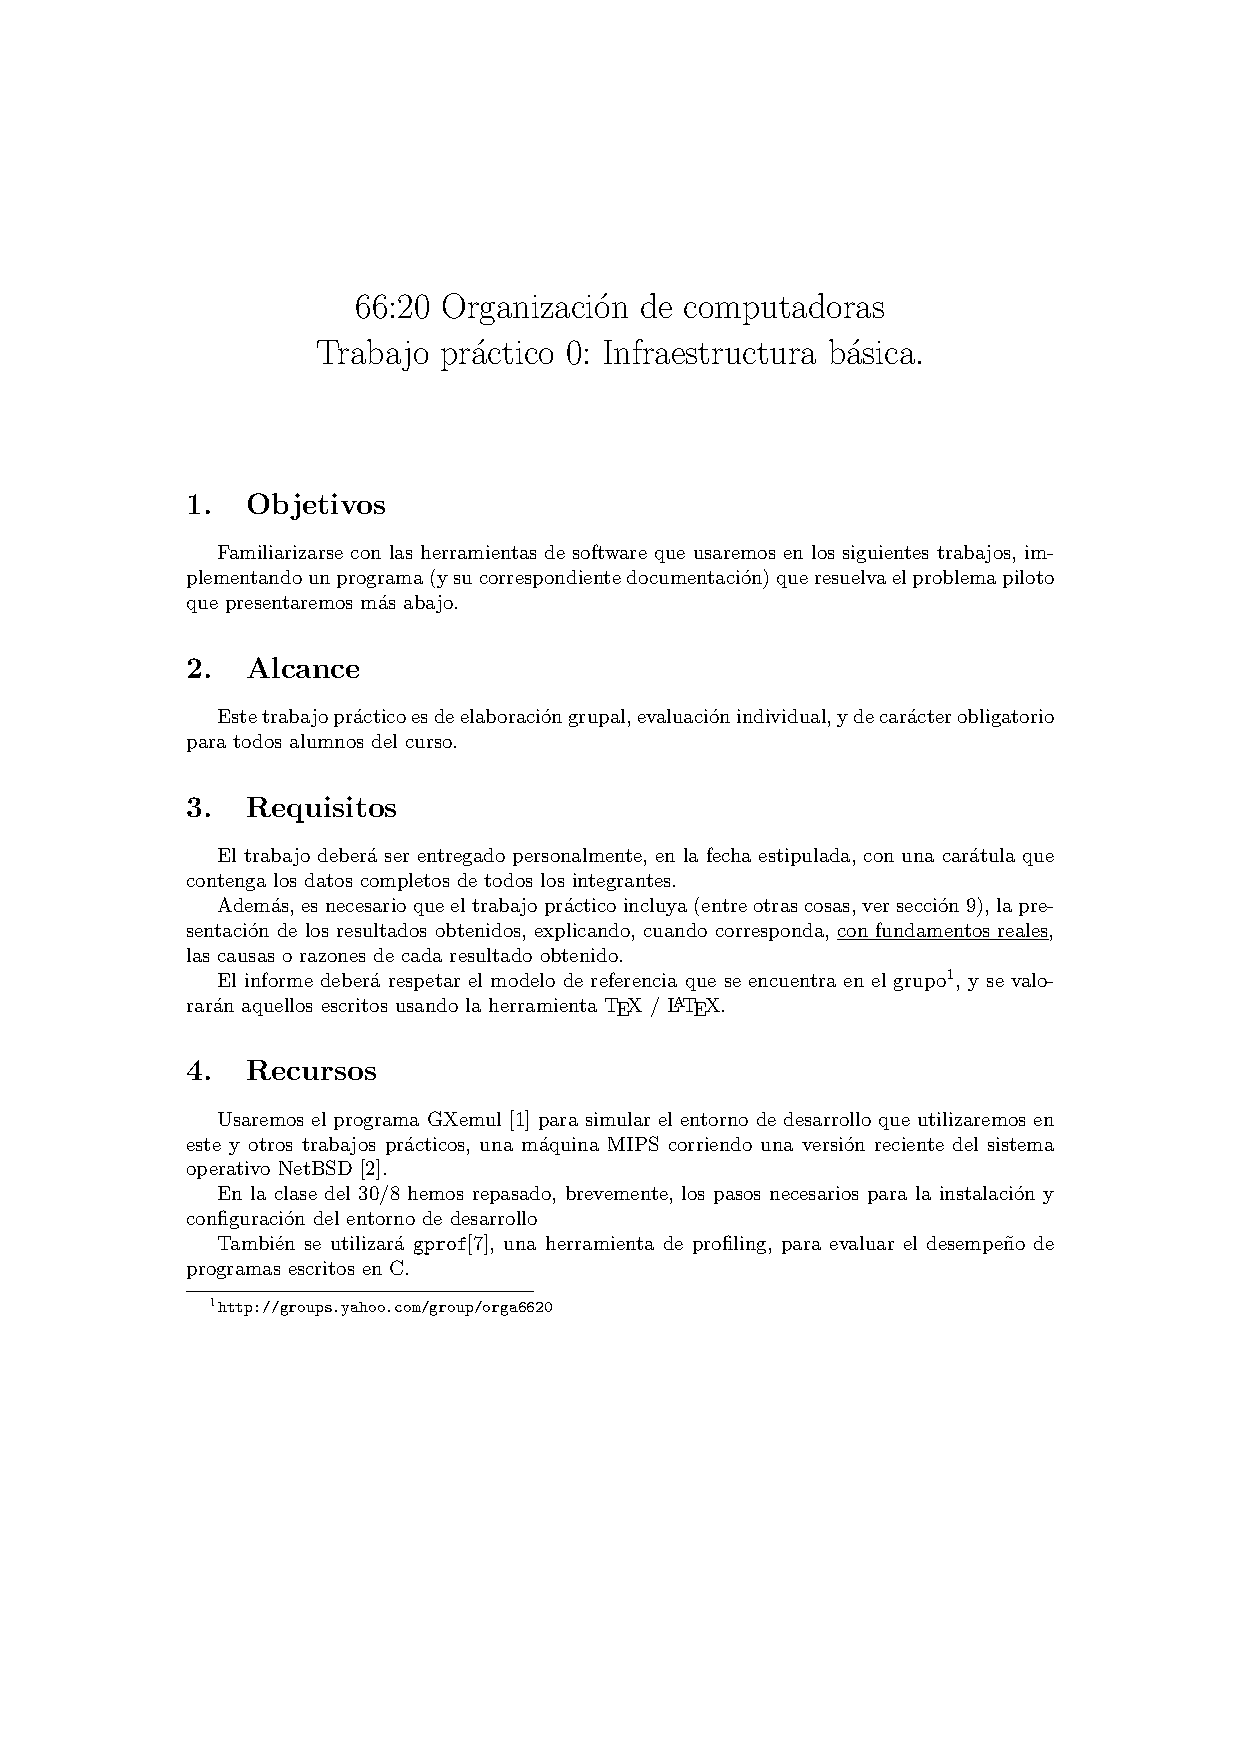
\includepdf[pages={-}]{docs/enunciado.pdf}

\end{document}
